\documentclass[12pt,a4paper,oneside]{book}

\usepackage[utf8]{inputenc}
\usepackage[english]{babel}
\usepackage{amssymb}
\usepackage{frontespizio}
\usepackage{enumitem}
\usepackage{fancyhdr}
\usepackage{eurosym}
\usepackage{graphicx}
\usepackage{xcolor}
\usepackage{minted}

\fancypagestyle{plain}{
	\fancyhf{}
	\fancyfoot[C]{\thepage}
	\renewcommand{\headrulewidth}{\ifnum\value{chapter}>0 0.5pt \else 0pt \fi}
	\renewcommand{\footrulewidth}{0pt}
	\fancyhead[L]{\ifnum\value{chapter}>0 \bfseries \itshape \nouppercase \leftmark \fi}
}

\pagestyle{plain}

\newcommand\itemtext[2]{
	\expandafter\gdef\csname item#1\endcsname{#2}
	\label{#1}#2}

\newcommand\refitemtext[1]{\csname item#1\endcsname}

\begin{document}
	
\begin{frontespizio}
	\Istituzione{Politecnico di Milano}
	\Logo[3cm]{logo.png}
	\Divisione{Computer Science and Engineering}
	\Scuola{}
	\Titoletto{Software Engineering 2}
	\Titolo{Design document}
	\Sottotitolo{\textbf{PowerEnJoy}}
	\NCandidato{Authors}
	\Candidato{Francesco Fabiani\\Jagadesh Manivannan\\Niccolò Pozzolini}
	\NRelatore{Professors}{}
	\Relatore{Elisabetta Di Nitto\\Luca Mottola}
	\Piede{Academic Year 2016/2017}
\end{frontespizio}
 
\tableofcontents

\chapter{Introduction}

\section{Purpose}
The Requirement Analysis and Specifications Document aims to provide in detail every aspect of the service PowerEnJoy, including its components, goals, constraints, functional and non-functional requirements. Use cases and scenarios for all the users involved will be provided as well to conform the product's objectives to the real world.

The last part of this document is reserved to the formalization of some features of the system involving the utilization of Alloy, a declarative specification language which provides a structural modeling tool based on first-order logic.

The high-level functionalities described in the RASD are intended for both developers and project managers. The former have to implement and test the functionalities while the latter must examine whether every requirement has been respected. It may also be useful to users in order to best take advantage of the service.

\section{Description of the problem}
The product described in this RASD is PowerEnJoy, a car-sharing service which offers to its users exclusively electric cars. It includes the common functionalities of its category: permitting to registered users to obtain the position of all the available cars, reserving one within a certain amount of time and continuously displaying the up-to-the-minute cost of the ride are just few of them. Moreover, PowerEnJoy stimulates users to behave virtuously towards the ecosystem by applying various types of discounts under specific conditions.

There are four software components that constitute the PowerEnJoy project. First, a back-end server provides APIs in order to simplify the communication related to the interactions of a user with the cars. Then two applications are available for a user to allow him/her the employment of every functionality: a web-based application (intended for visualization from desktop) and a mobile one. Lastly, every vehicle will be equipped with an on-board computer, used by the driver to manage the ride with the available options and see real-time information related to it, such as the time spent, the distance traveled and the total amount.

\section{Goals}
\begin{enumerate}[label={[G\arabic*]},labelindent=\parindent,leftmargin=*]
	\item \label{goal:registration} Registration of a user to the system
	\item \label{goal:cars_location} Finding the locations of the available cars
	\item \label{goal:reservation} Reservation of a car
	\item \label{goal:expiration} Expiration of reservation and penalization
	\item \label{goal:entry} Entry of registered user into the car
	\item \label{goal:charging} Start charging and notifying the registered user
	\item \label{goal:car_locking} Stop charging the registered user and lock the car
	\item \label{goal:safe_areas} Safe areas for parking the reserved cars
	\item \label{goal:passengers} Detection of extra passengers and applying discount
	\item \label{goal:battery} Detection of the battery status and applying discount
	\item \label{goal:special_areas} Detection of special parking areas and applying discount
	\item \label{goal:constraints} Checking parking and battery constraints and penalization
\end{enumerate}

\section{Domain properties}
\begin{itemize}
	\item User's data are always valid
	\item Location reported by the GPS is always accurate
	\item Every user can reserve just a car per time
\end{itemize}

\section{Glossary}

\subsection{Definitions}
\begin{itemize}
	\item \emph{Car}: electric vehicle provided by the service
	\item \emph{Guest} or \emph{Guest user}: person not registered to the service
	\item \emph{Registered user}: see \emph{User}
	\item \emph{Safe area}: set of parking spots where a user can leave a car without penalization 
	\item \emph{User}: person with a valid driving license registered to the service
\end{itemize}

\subsection{Acronyms}
\begin{itemize}
	\item \emph{API}: Application Programming Interface
	\item \emph{GPS}: Global Positioning System
	\item \emph{OS}: Operating System, related both to desktop and mobile platforms
	\item \emph{PIN}: Personal Identification Number
	\item \emph{RASD}: Requirements Analysis and Specification Document
	\item \emph{W3C}: World Wide Web Consortium
\end{itemize}

\section{Constrains}

\subsection{Regulatory policies}
While waiting for future conventions, at the moment toll and handicap parkings are forbidden. Timed parkings are also forbidden, since the user cannot ensure compliance with the deadline once left the car.

During the registration the system receive the user's permission to get his position and it has to handle sensible data according to the privacy law. To avoid SPAM the system can only use messages and notifications if strictly required to the proper operation of the system.

\subsection{Hardware limitations}
\begin{itemize}
	\item User's mobile device:
\begin{itemize}
	\item Connection speed \(\geqslant\) 3G
	\item GPS
	\item Enough memory available to install the app
\end{itemize}
	\item Car:
	\begin{itemize}
	\item GPS
	\item Weight sensor for each seat
	\item Fast Internet connection
	\item On-board computer with integrated system
\end{itemize}
\end{itemize}

\subsection{Interfaces to other applications}
Interface with an SMS gateway provider via standard SMS REST APIs, to verify the user's account and send important notifications.

\subsection{Parallel operation}
The server supports parallel reservations of cars from different users at the same time.

\section{Reference documents}
The Requirements Analysis and Specification Document has been composed following the indications and examples reported in the document ISO/IEC/ IEEE 29148, released by W3C, containing provisions for the processes and products related to the engineering of requirements for systems and software products and services throughout the life cycle.

With regards to the course named Software Engineering II and held by professors Luca Mottola and Elisabetta Di Nitto (Politecnico di Milano, a.~y. 2016/17), the document conforms to the guidelines provided during the lectures and within the material of the course.
\chapter{Architectural design}

\section{Overview}

\section{Component view}

\section{Deployment view}
\begin{figure}[h]
	\centering
	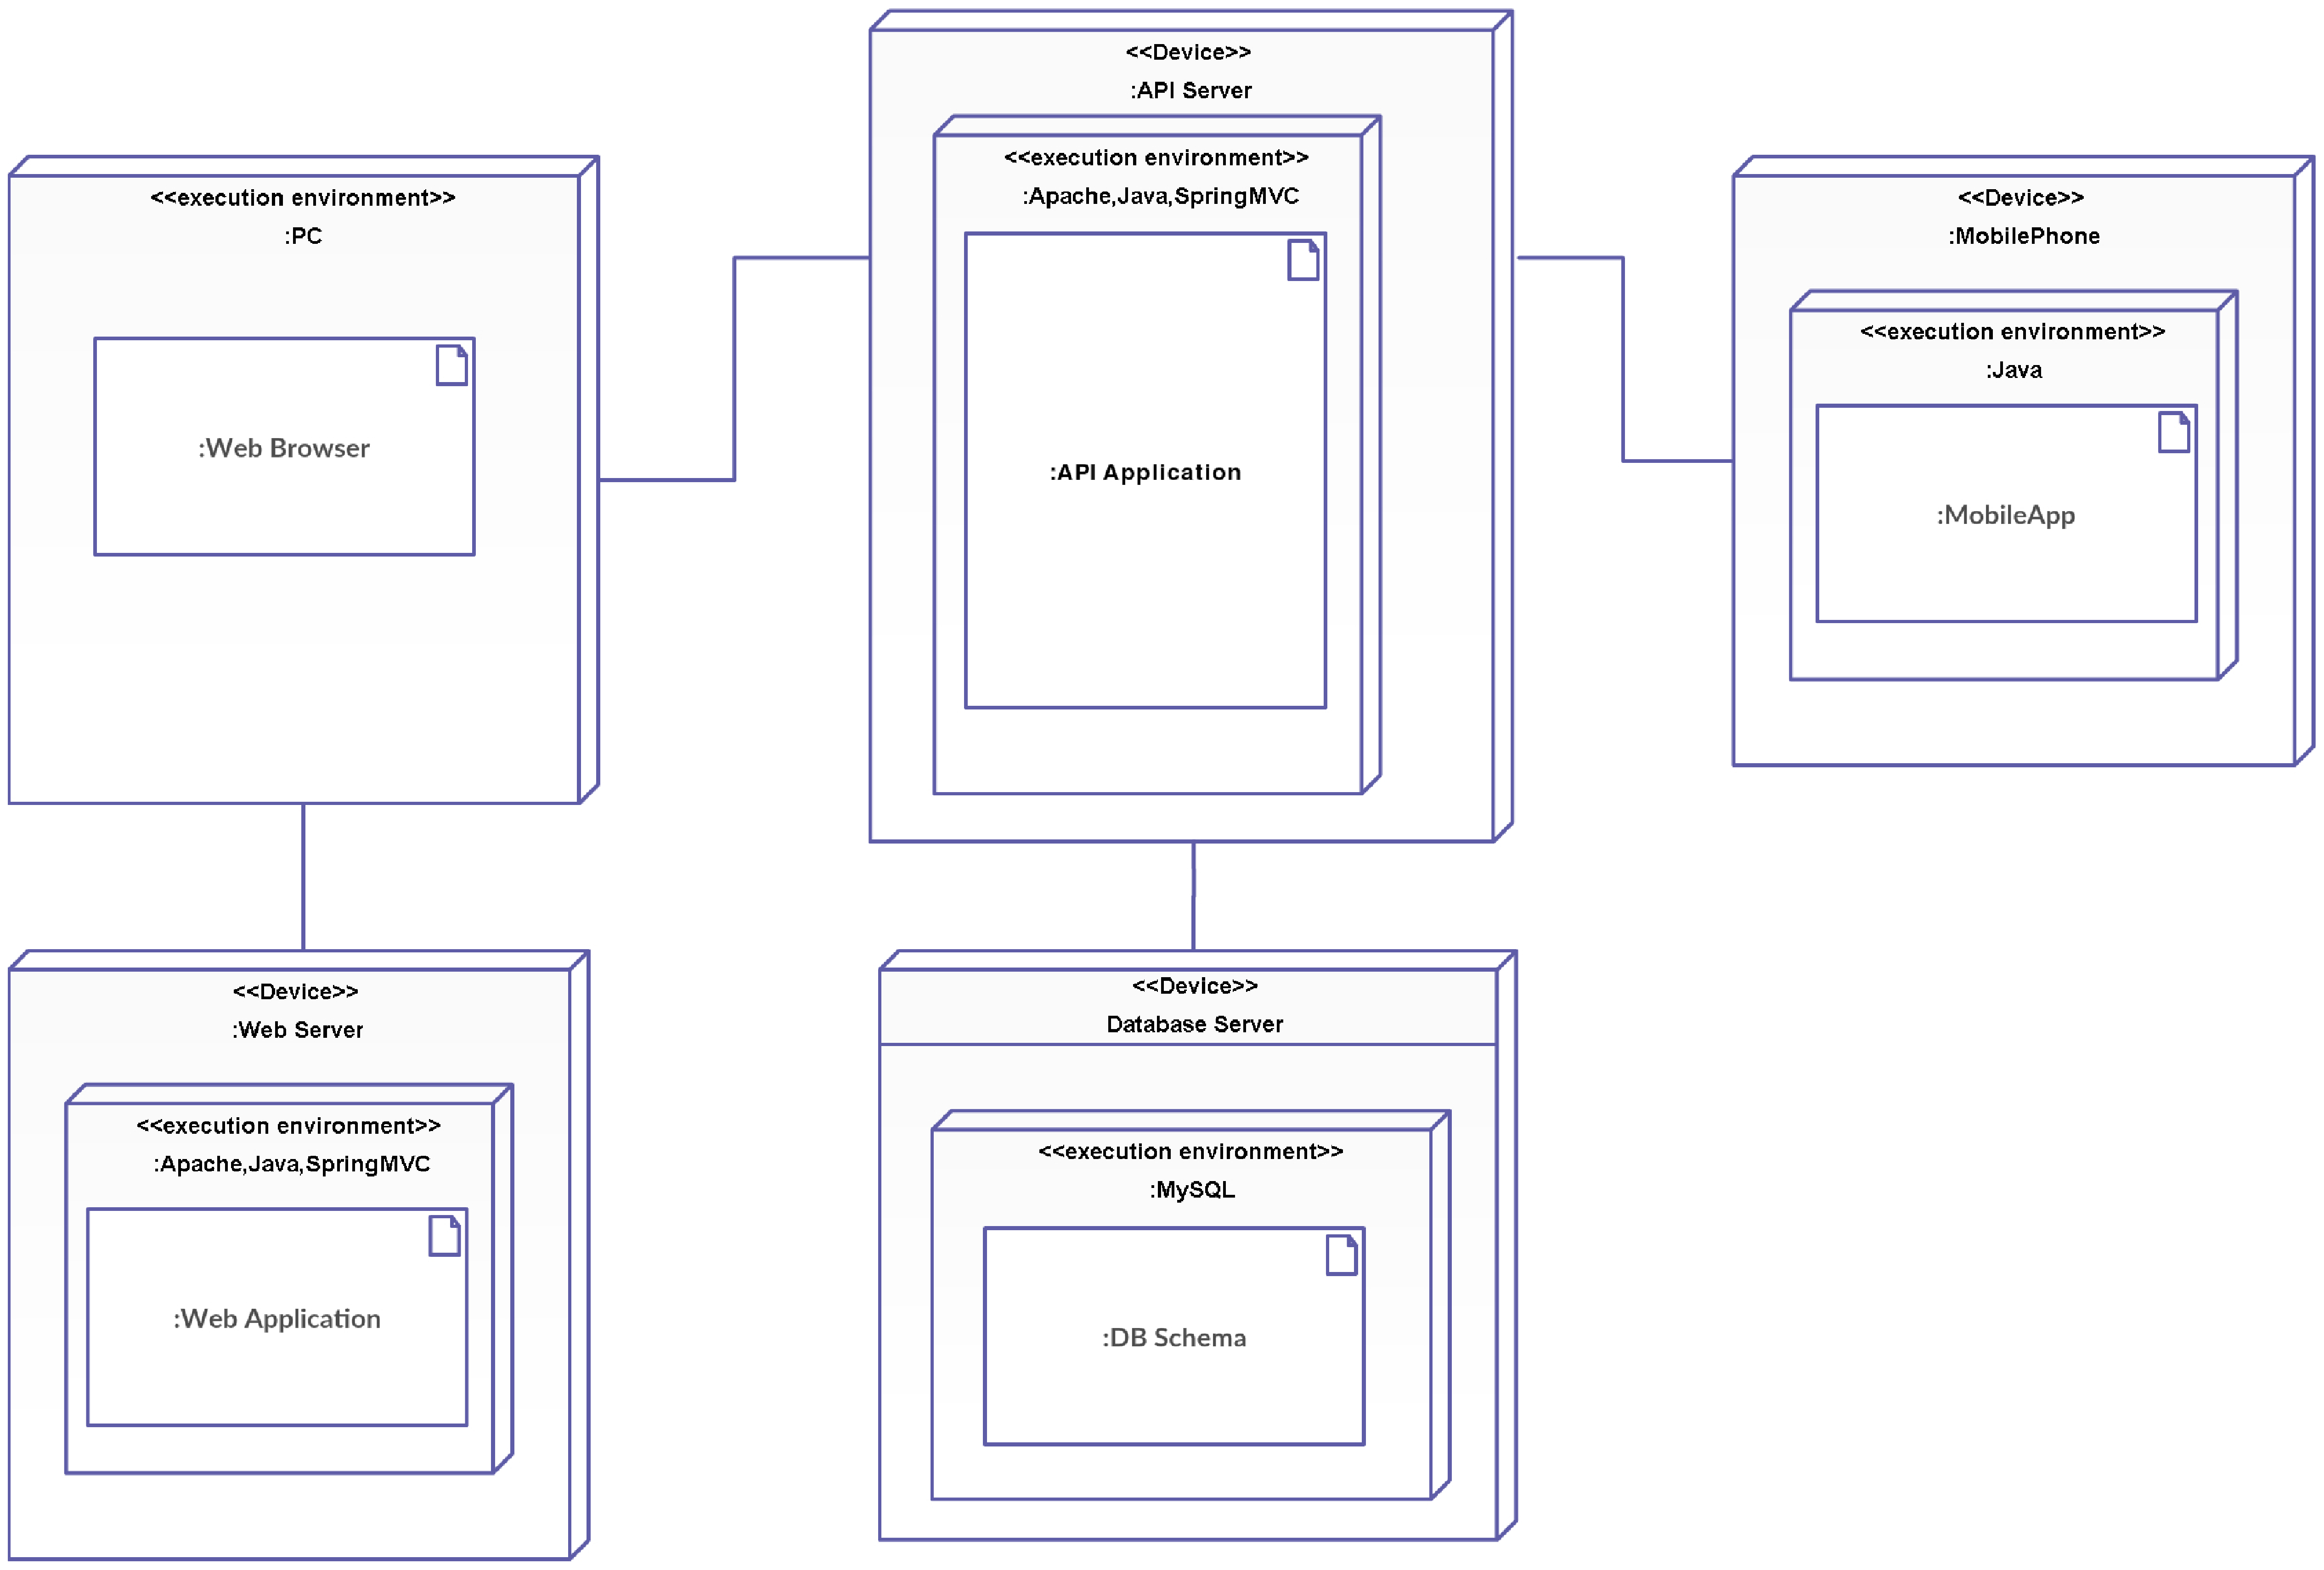
\includegraphics[width=\linewidth,keepaspectratio]{figures/deployment_view.eps}
	\caption{Deployment view diagram of the system}
	\label{fig:deployment_view}
\end{figure}

\section{Runtime view}
This section describes the system components involved and the related interactions for some of the use cases reported in the RASD.

Map Manager:
This map manager is an interface that acts as a router to communicate between the Client/User and with the system. In the run time view sequence diagram,
the map manager is not shown mostly in all the diagrams. But in the individual explanation of the sequence diagram, its functionality is explained.

Components:
Each and every component are separated for specific functionality. This is done in order to achieve better performance and re-usability of the code.

\subsubsection{Selection of available car}
\begin{figure}[h]
	\centering
	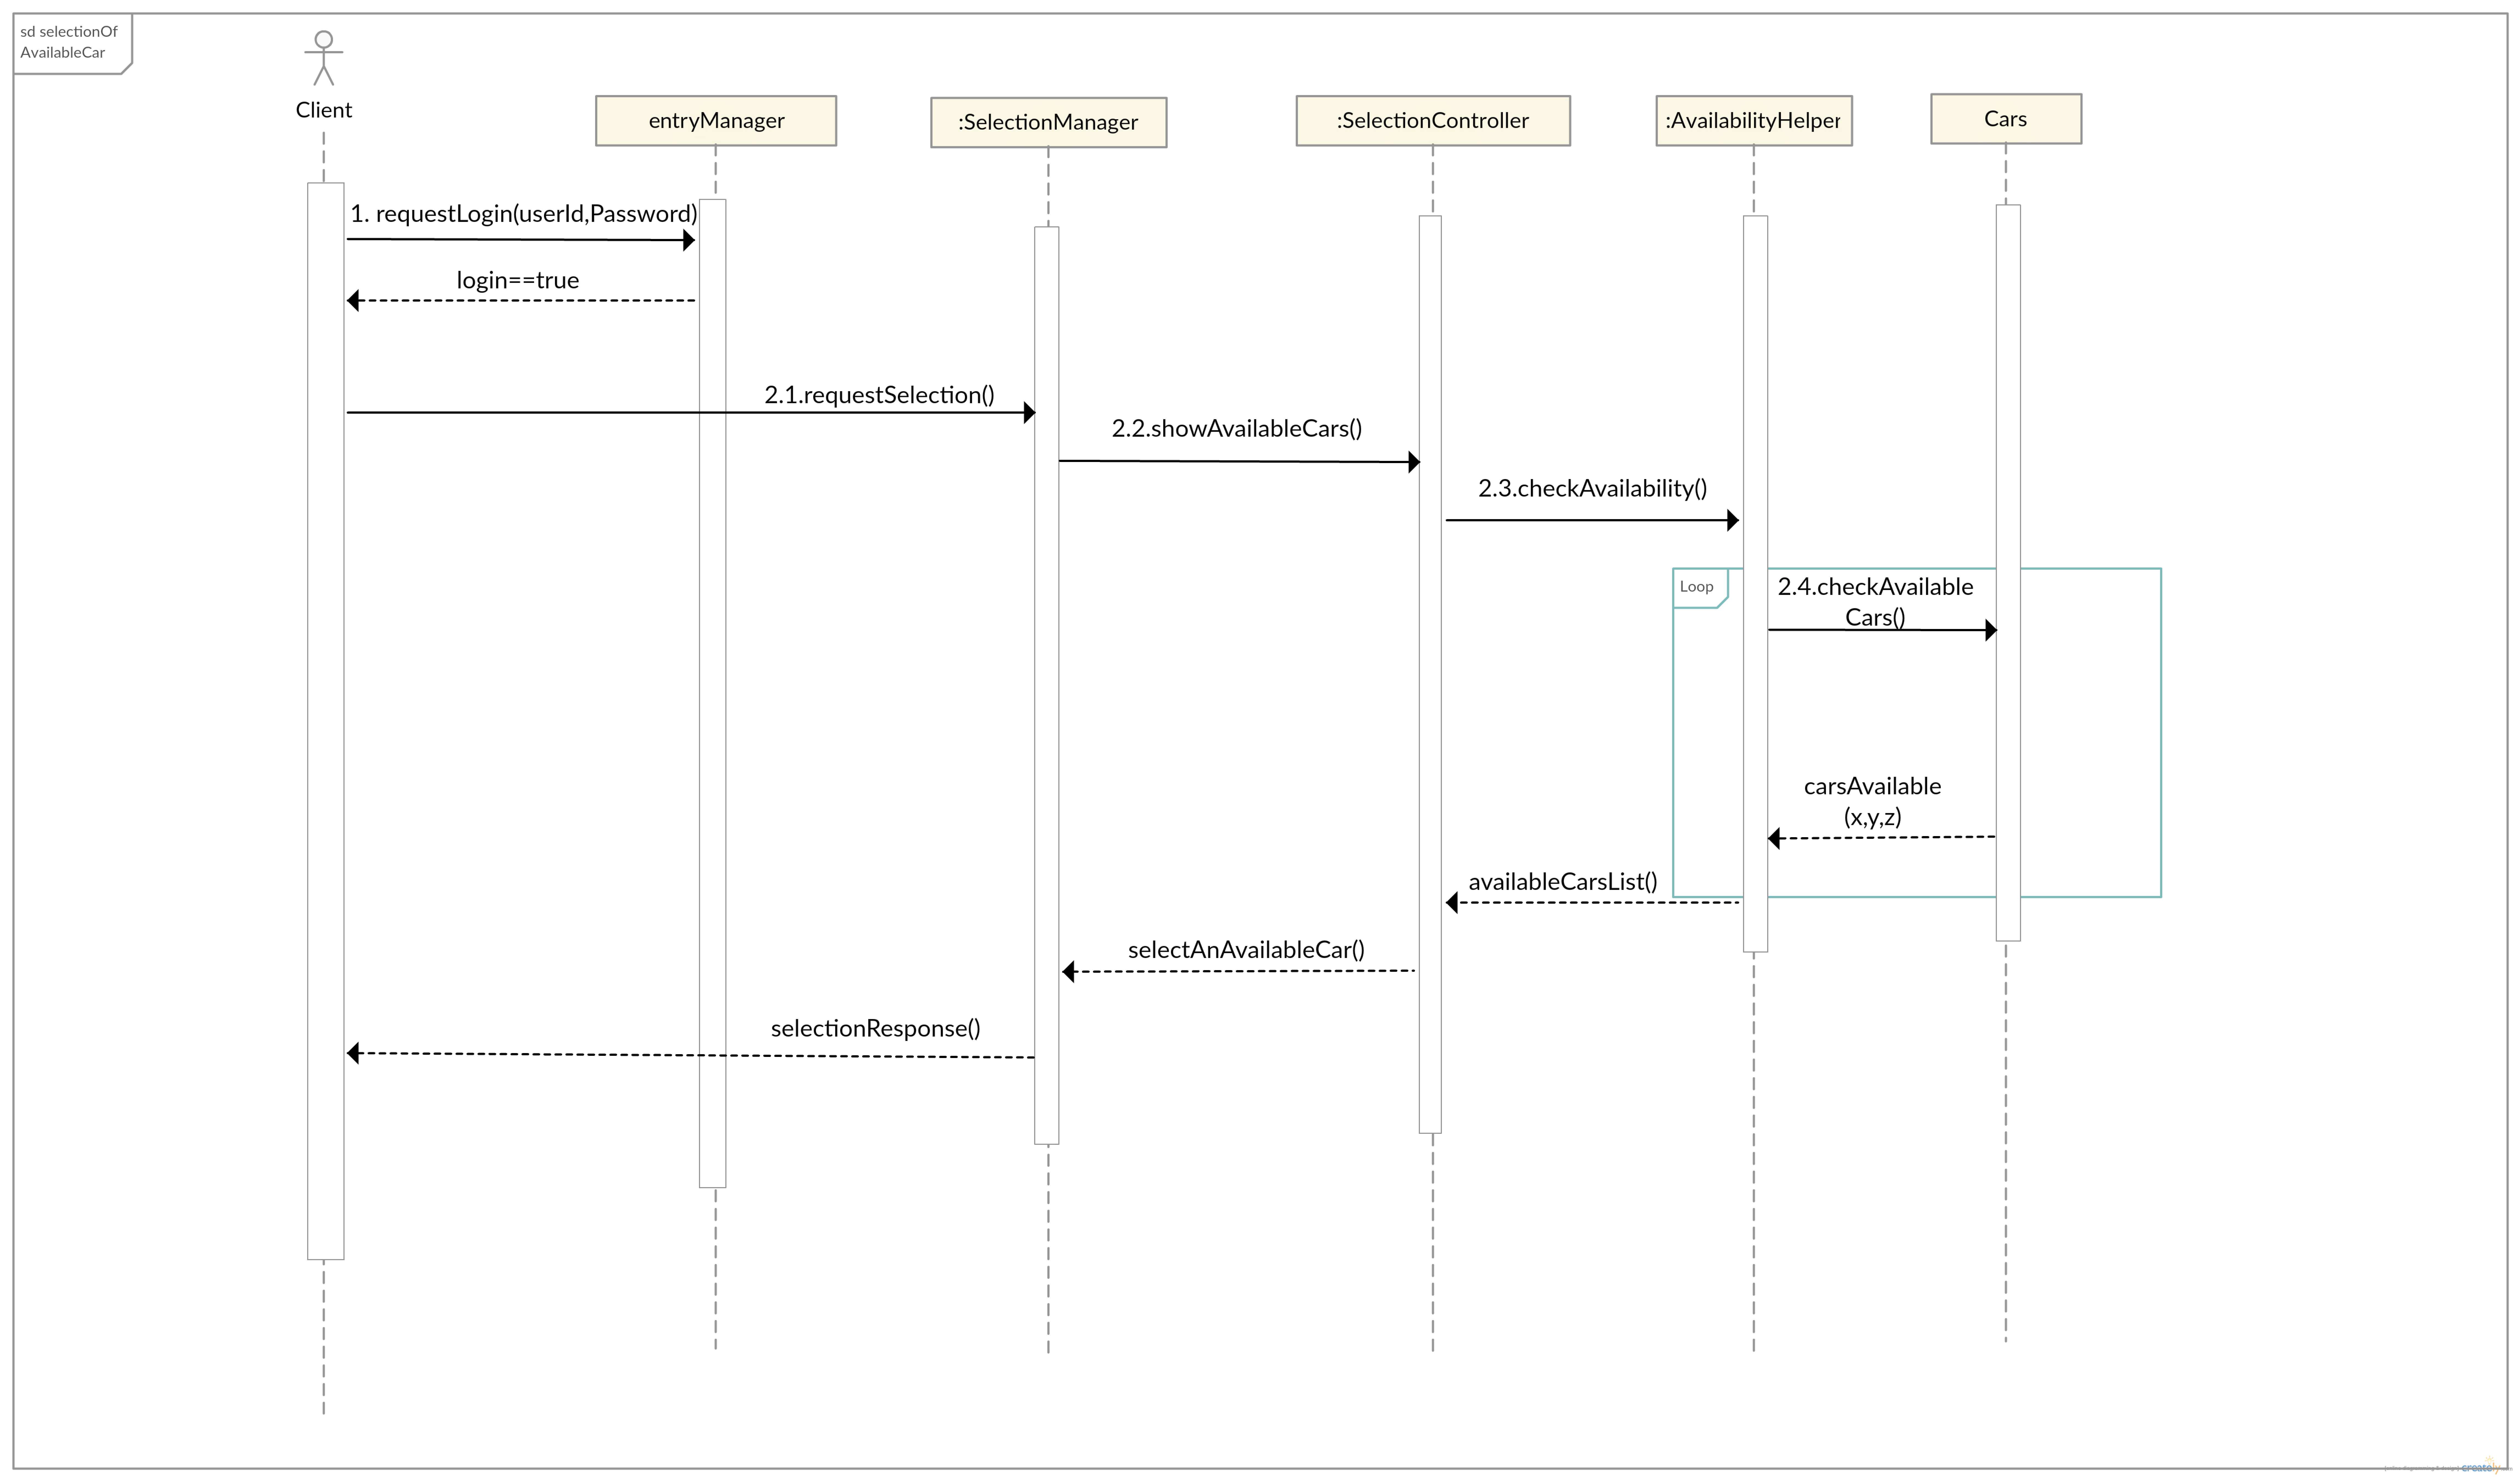
\includegraphics[width=\linewidth,keepaspectratio]{figures/selection_available_car_runtime.eps}
	\caption{Sequence diagram for the selection of the available car}
	\label{fig:selection_available_car_runtime}
\end{figure}

The Client/User wants to select an available car. Only after successful login, the Client/User will be able to select the car. A Login manager takes care of this credential verification.
After successful verification of the user credentials, the Client/User can send a request to select an available Car through the map manager which transfers the request to the selection
manager. This indeed interacts with the selection controller to display the list of available cars.

The controller interacts with another component called availability helper.
This availability helper communicates with all the cars and checks which cars are available. This check happens in a loop continuously After finding the list of available cars, then the response is transferred selection controller and finally it is transferred to the Client/User. After this, the user/client can select only one available car for the reservation.

\subsubsection{Reservation of selected car}
\begin{figure}[h]
	\centering
	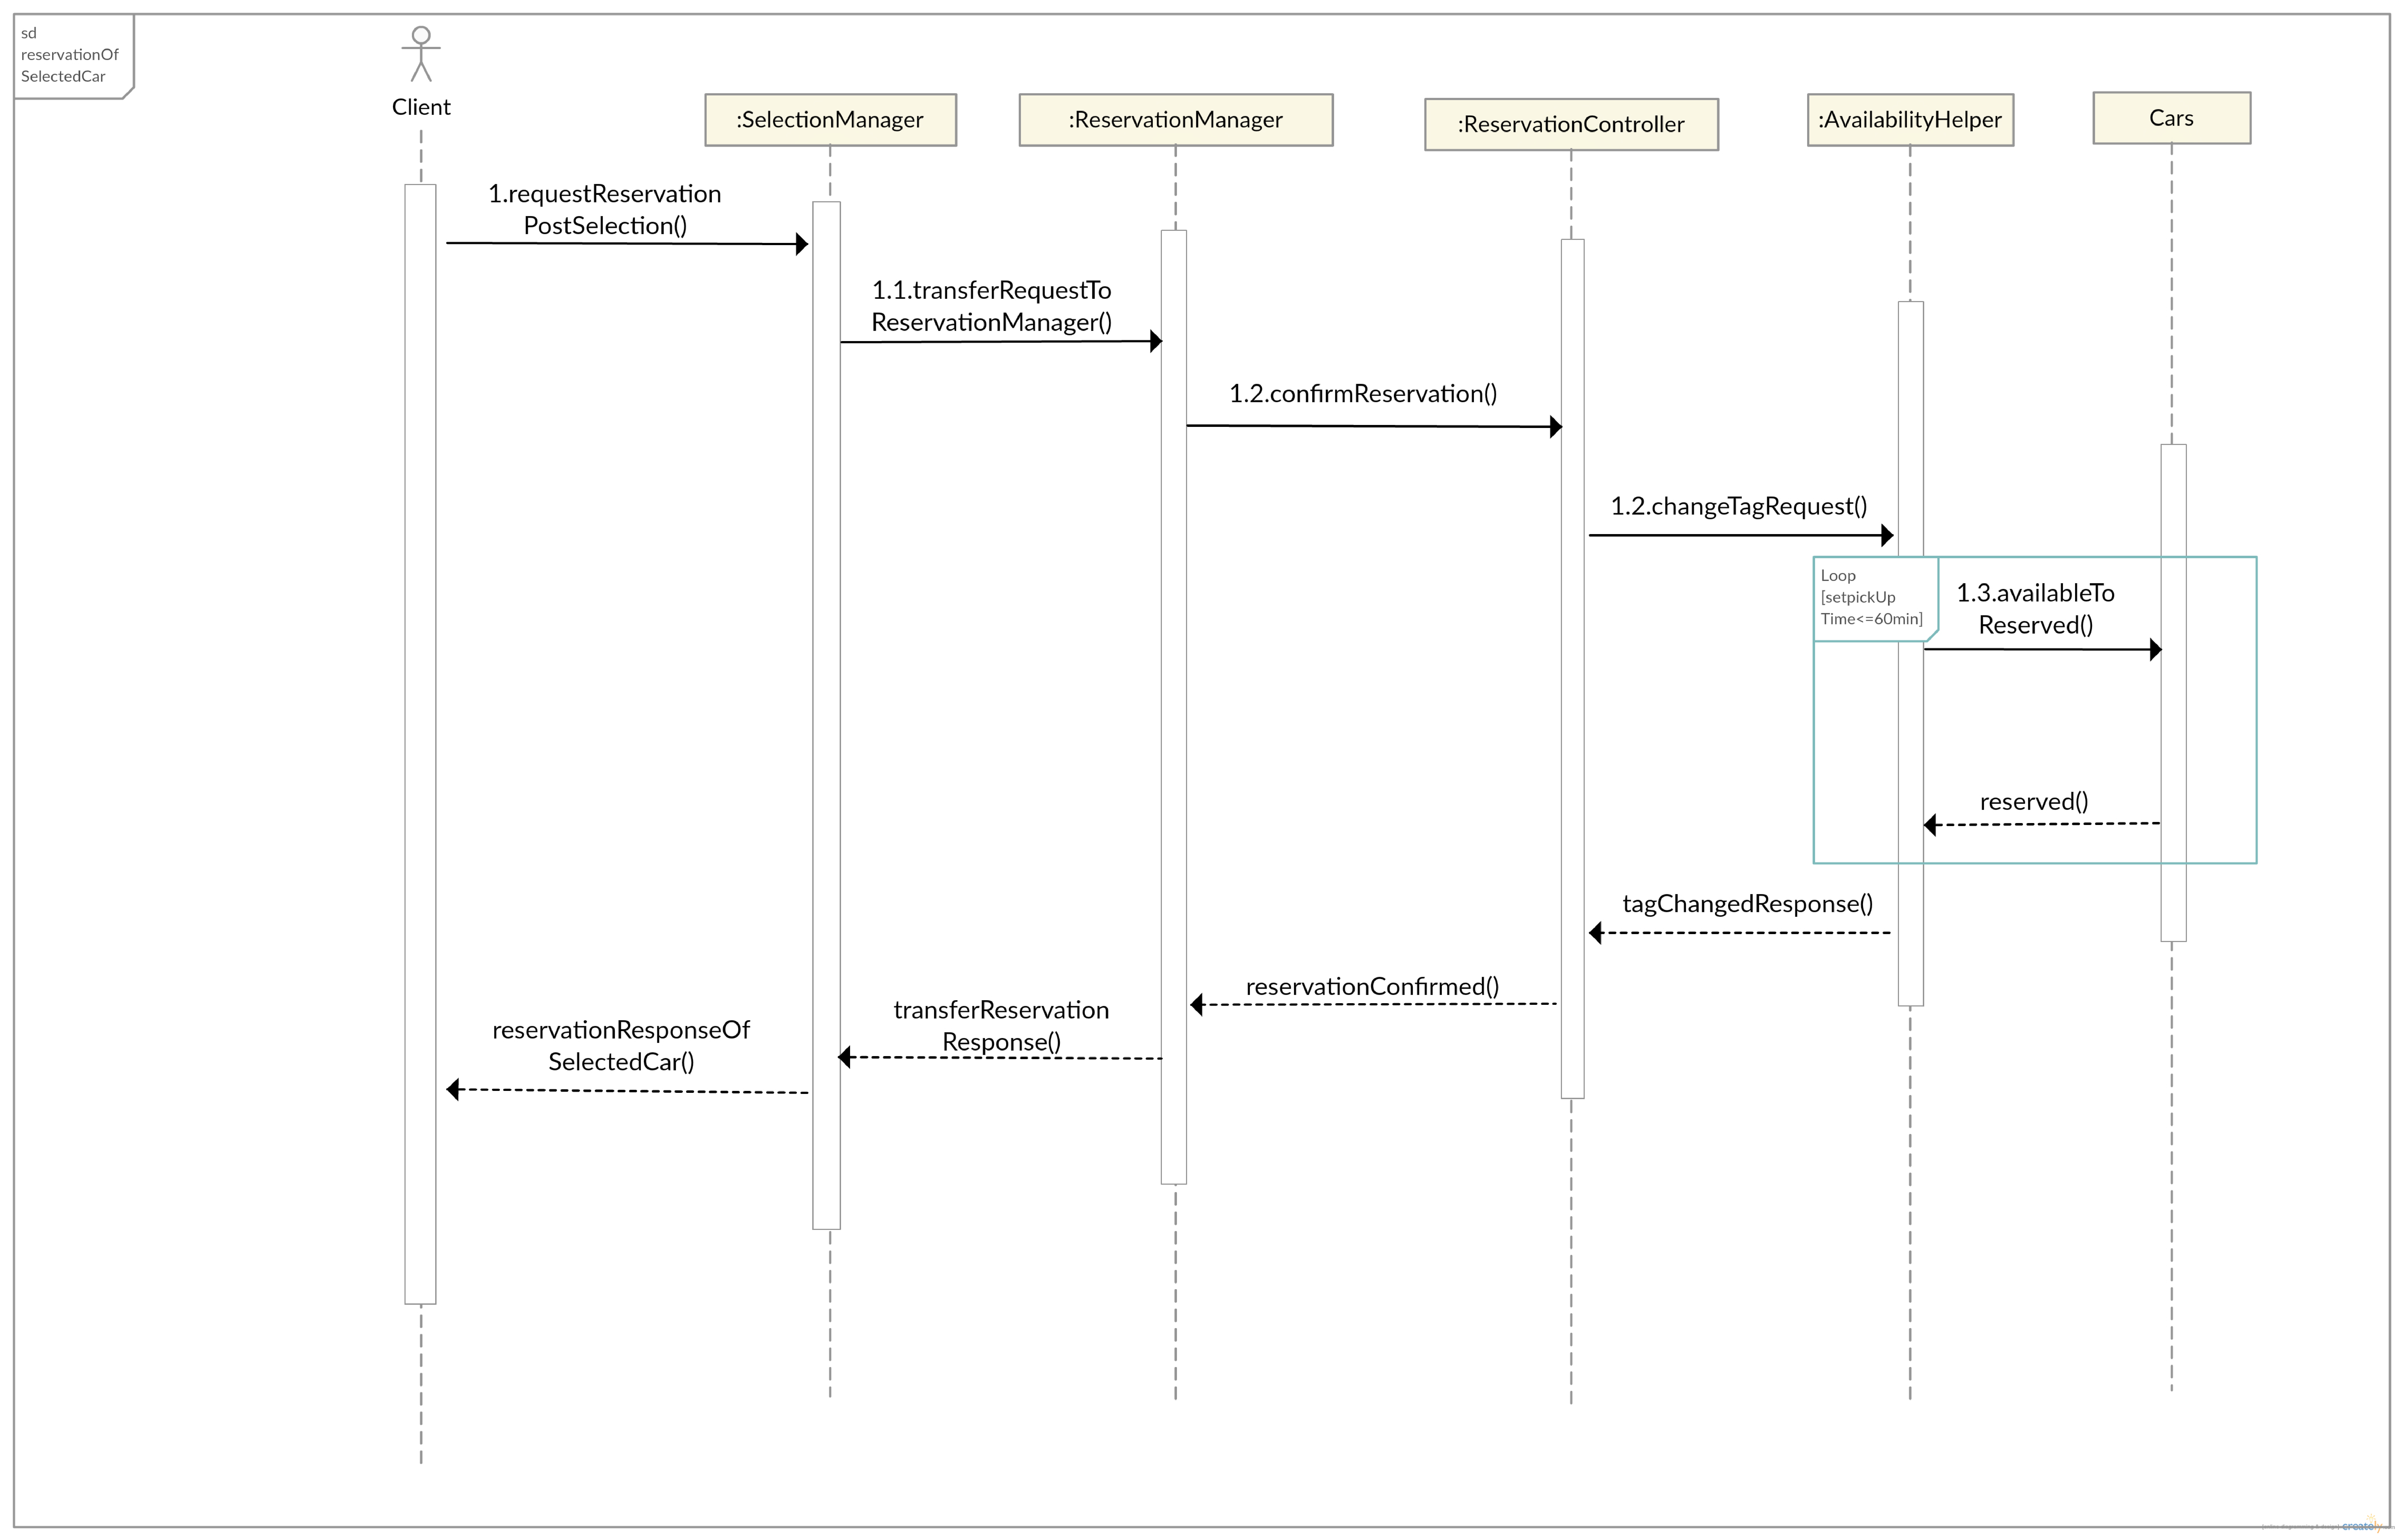
\includegraphics[width=\linewidth,keepaspectratio]{figures/reservation_runtime.eps}
	\caption{Sequence diagram for the reservation of the selected car}
	\label{fig:reservation_runtime}
\end{figure}

The reservation confirmation of a car can happen only after selection of the available car. So the sequence of the user's request for the reservation starts from the selection manager. It transfers the request to the reservation manager for the confirmation. The reservation controller is a component that sends another request to the availability helper
to change the tag of the car selected.

The availability helper interacts with the car and changes the tag as ``reserved''. The availability helper starts a counter timer immediately after changing the tag by setting a time for 60 minutes. This tag will hold reserved only for upto 60 minutes. Now, the response is sent back to the reservation controller which is finally sent to the Client/User as a confirmed reservation.

\subsubsection{Selection of special parking areas}
\begin{figure}[h]
	\centering
	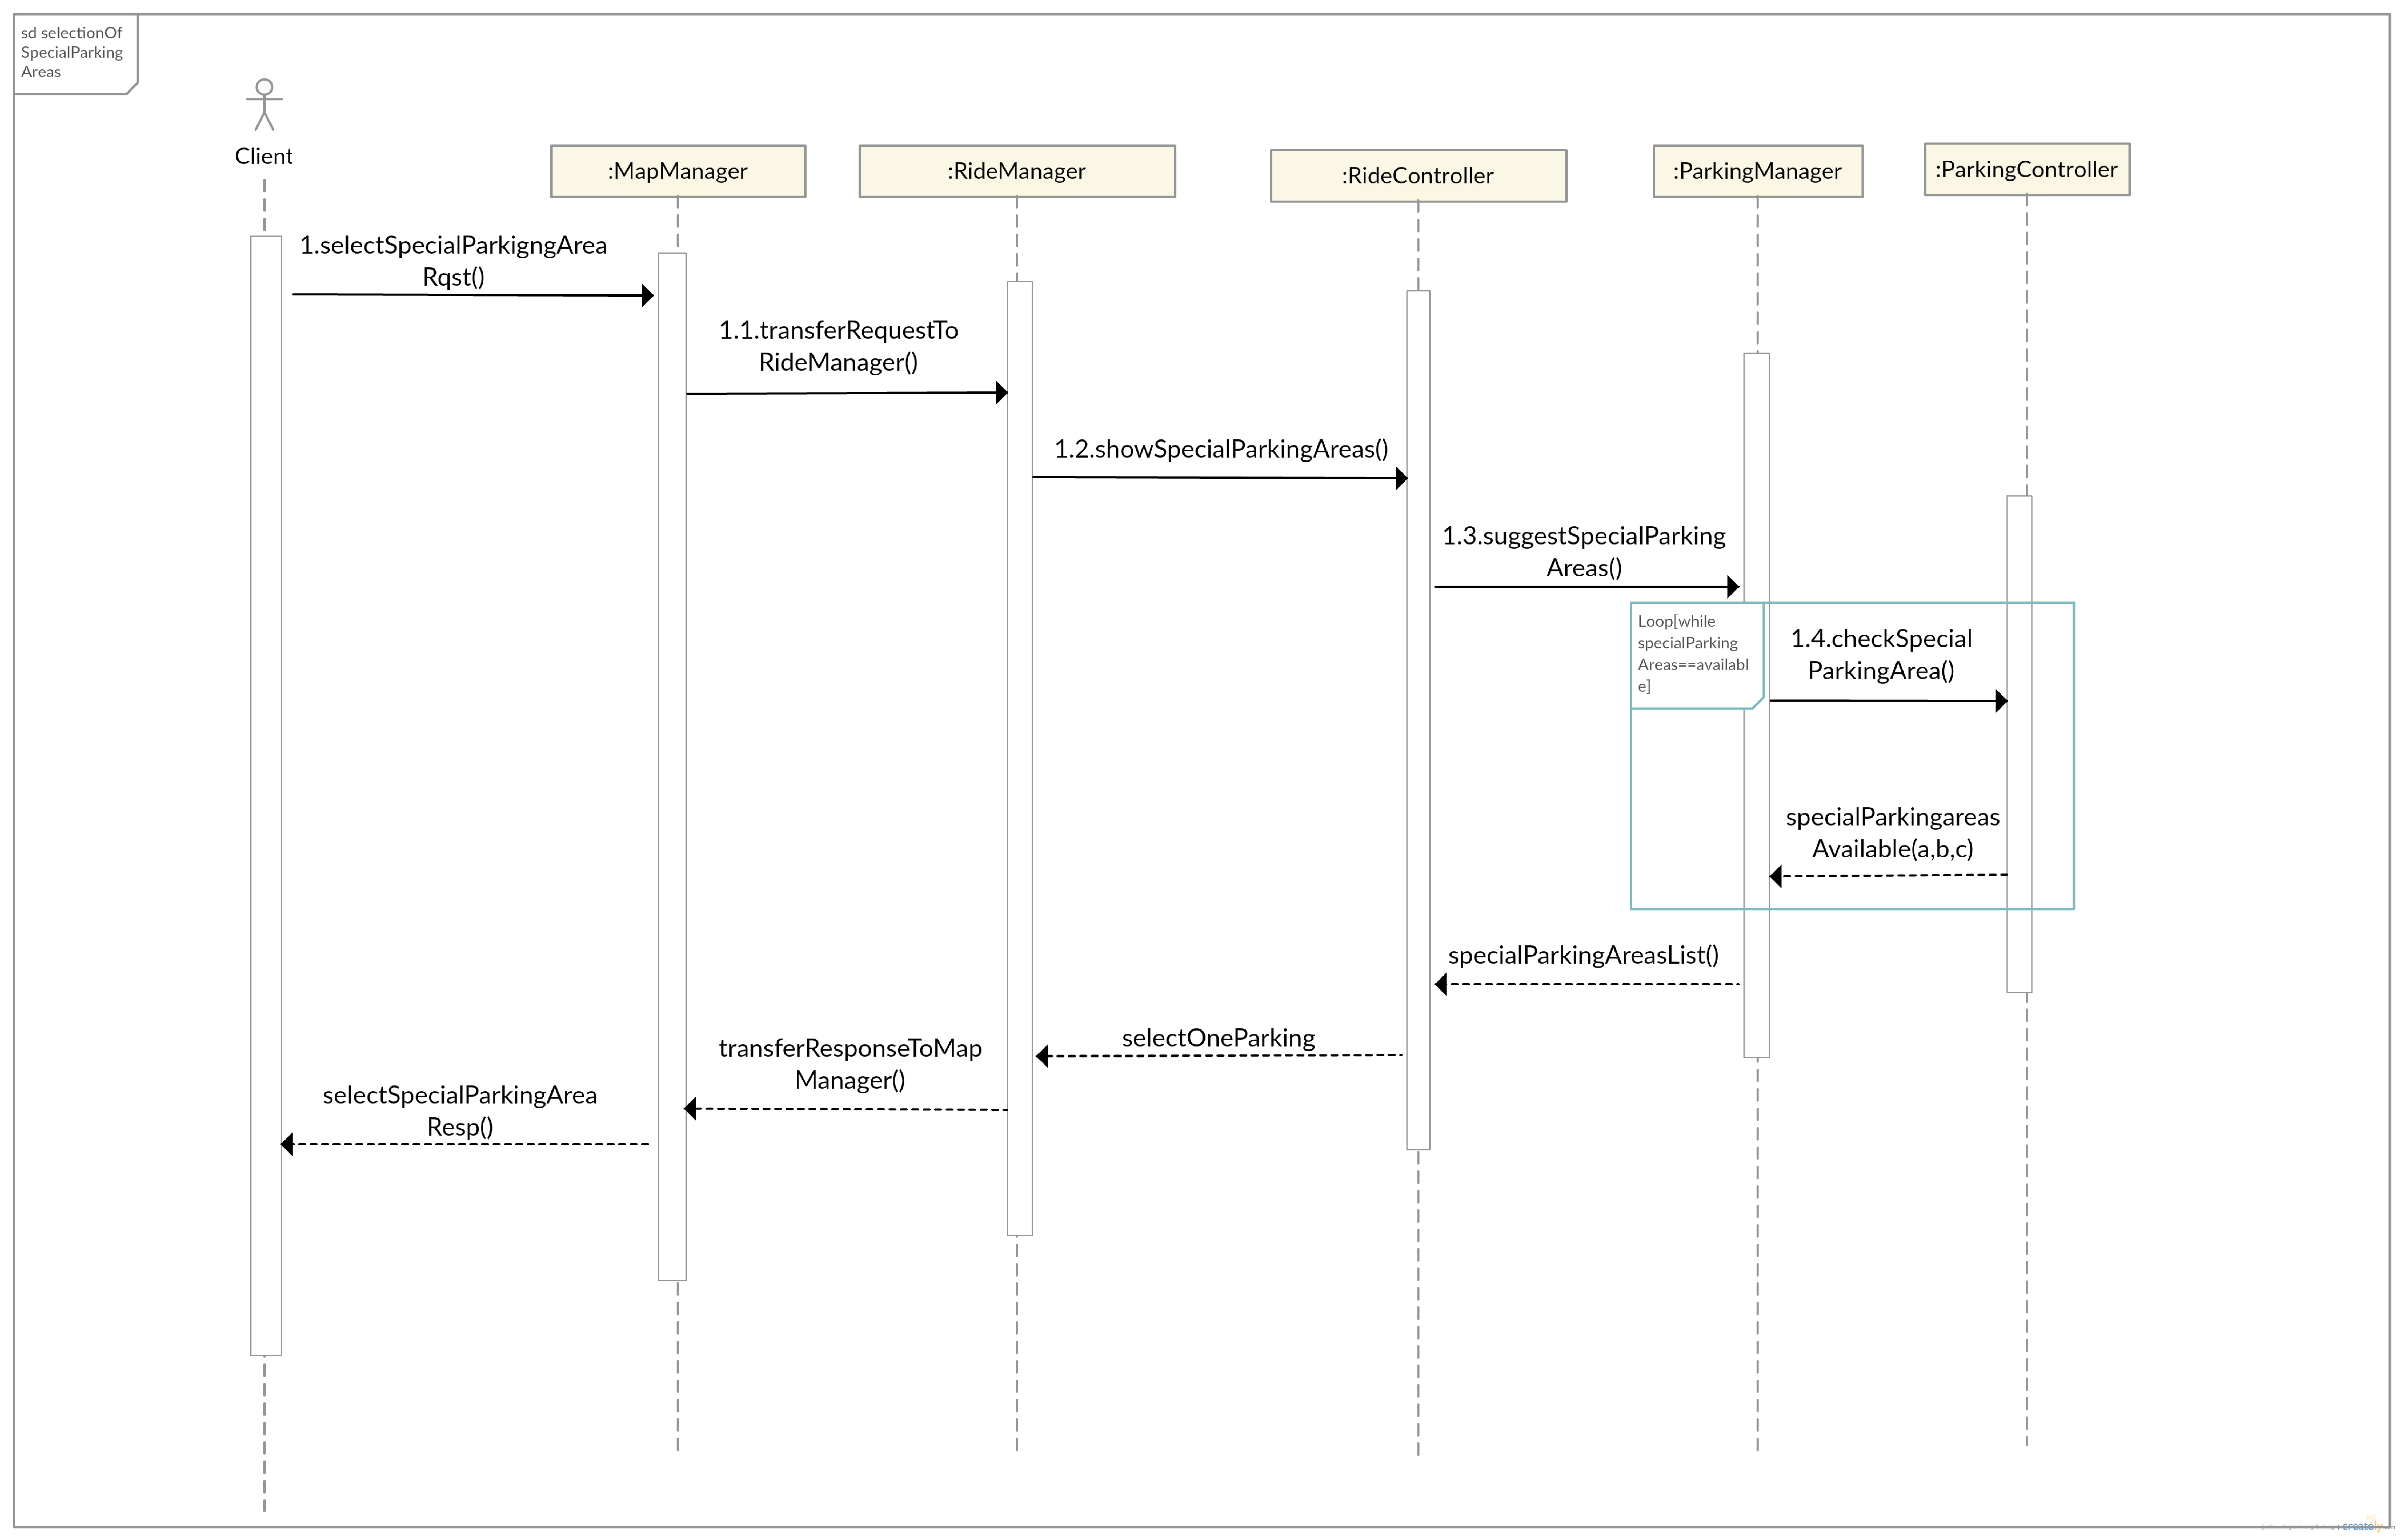
\includegraphics[width=\linewidth,keepaspectratio]{figures/special_parking_area_runtime.eps}
	\caption{Sequence diagram for the selection of special parking areas}
	\label{fig:special_parking_area_runtime}
\end{figure}

The Client/User requests for a special parking area to get a discount. So, he/she selects the option during the ride to the system through the map manager. The map manager
acts as an interface and transfers the request to the ride manager. The ride manager provides an interface to communicate with the ride controller during the ride. 

This component asks to display the available list of special parking areas nearby. So, the parking manager accepts this request while the parking controller checks the availability of special parking areas and sends the list of available special parking areas to the Parking manager. The parking controller does a check continuously in a loop. If there are no special parking areas available, then it sends an response with result as zero and suggests list of safe parking areas to the parking manager. This requests are finally sent as a response to the user/client.

\subsubsection{Enable money saving option for discount}
\begin{figure}[h]
	\centering
	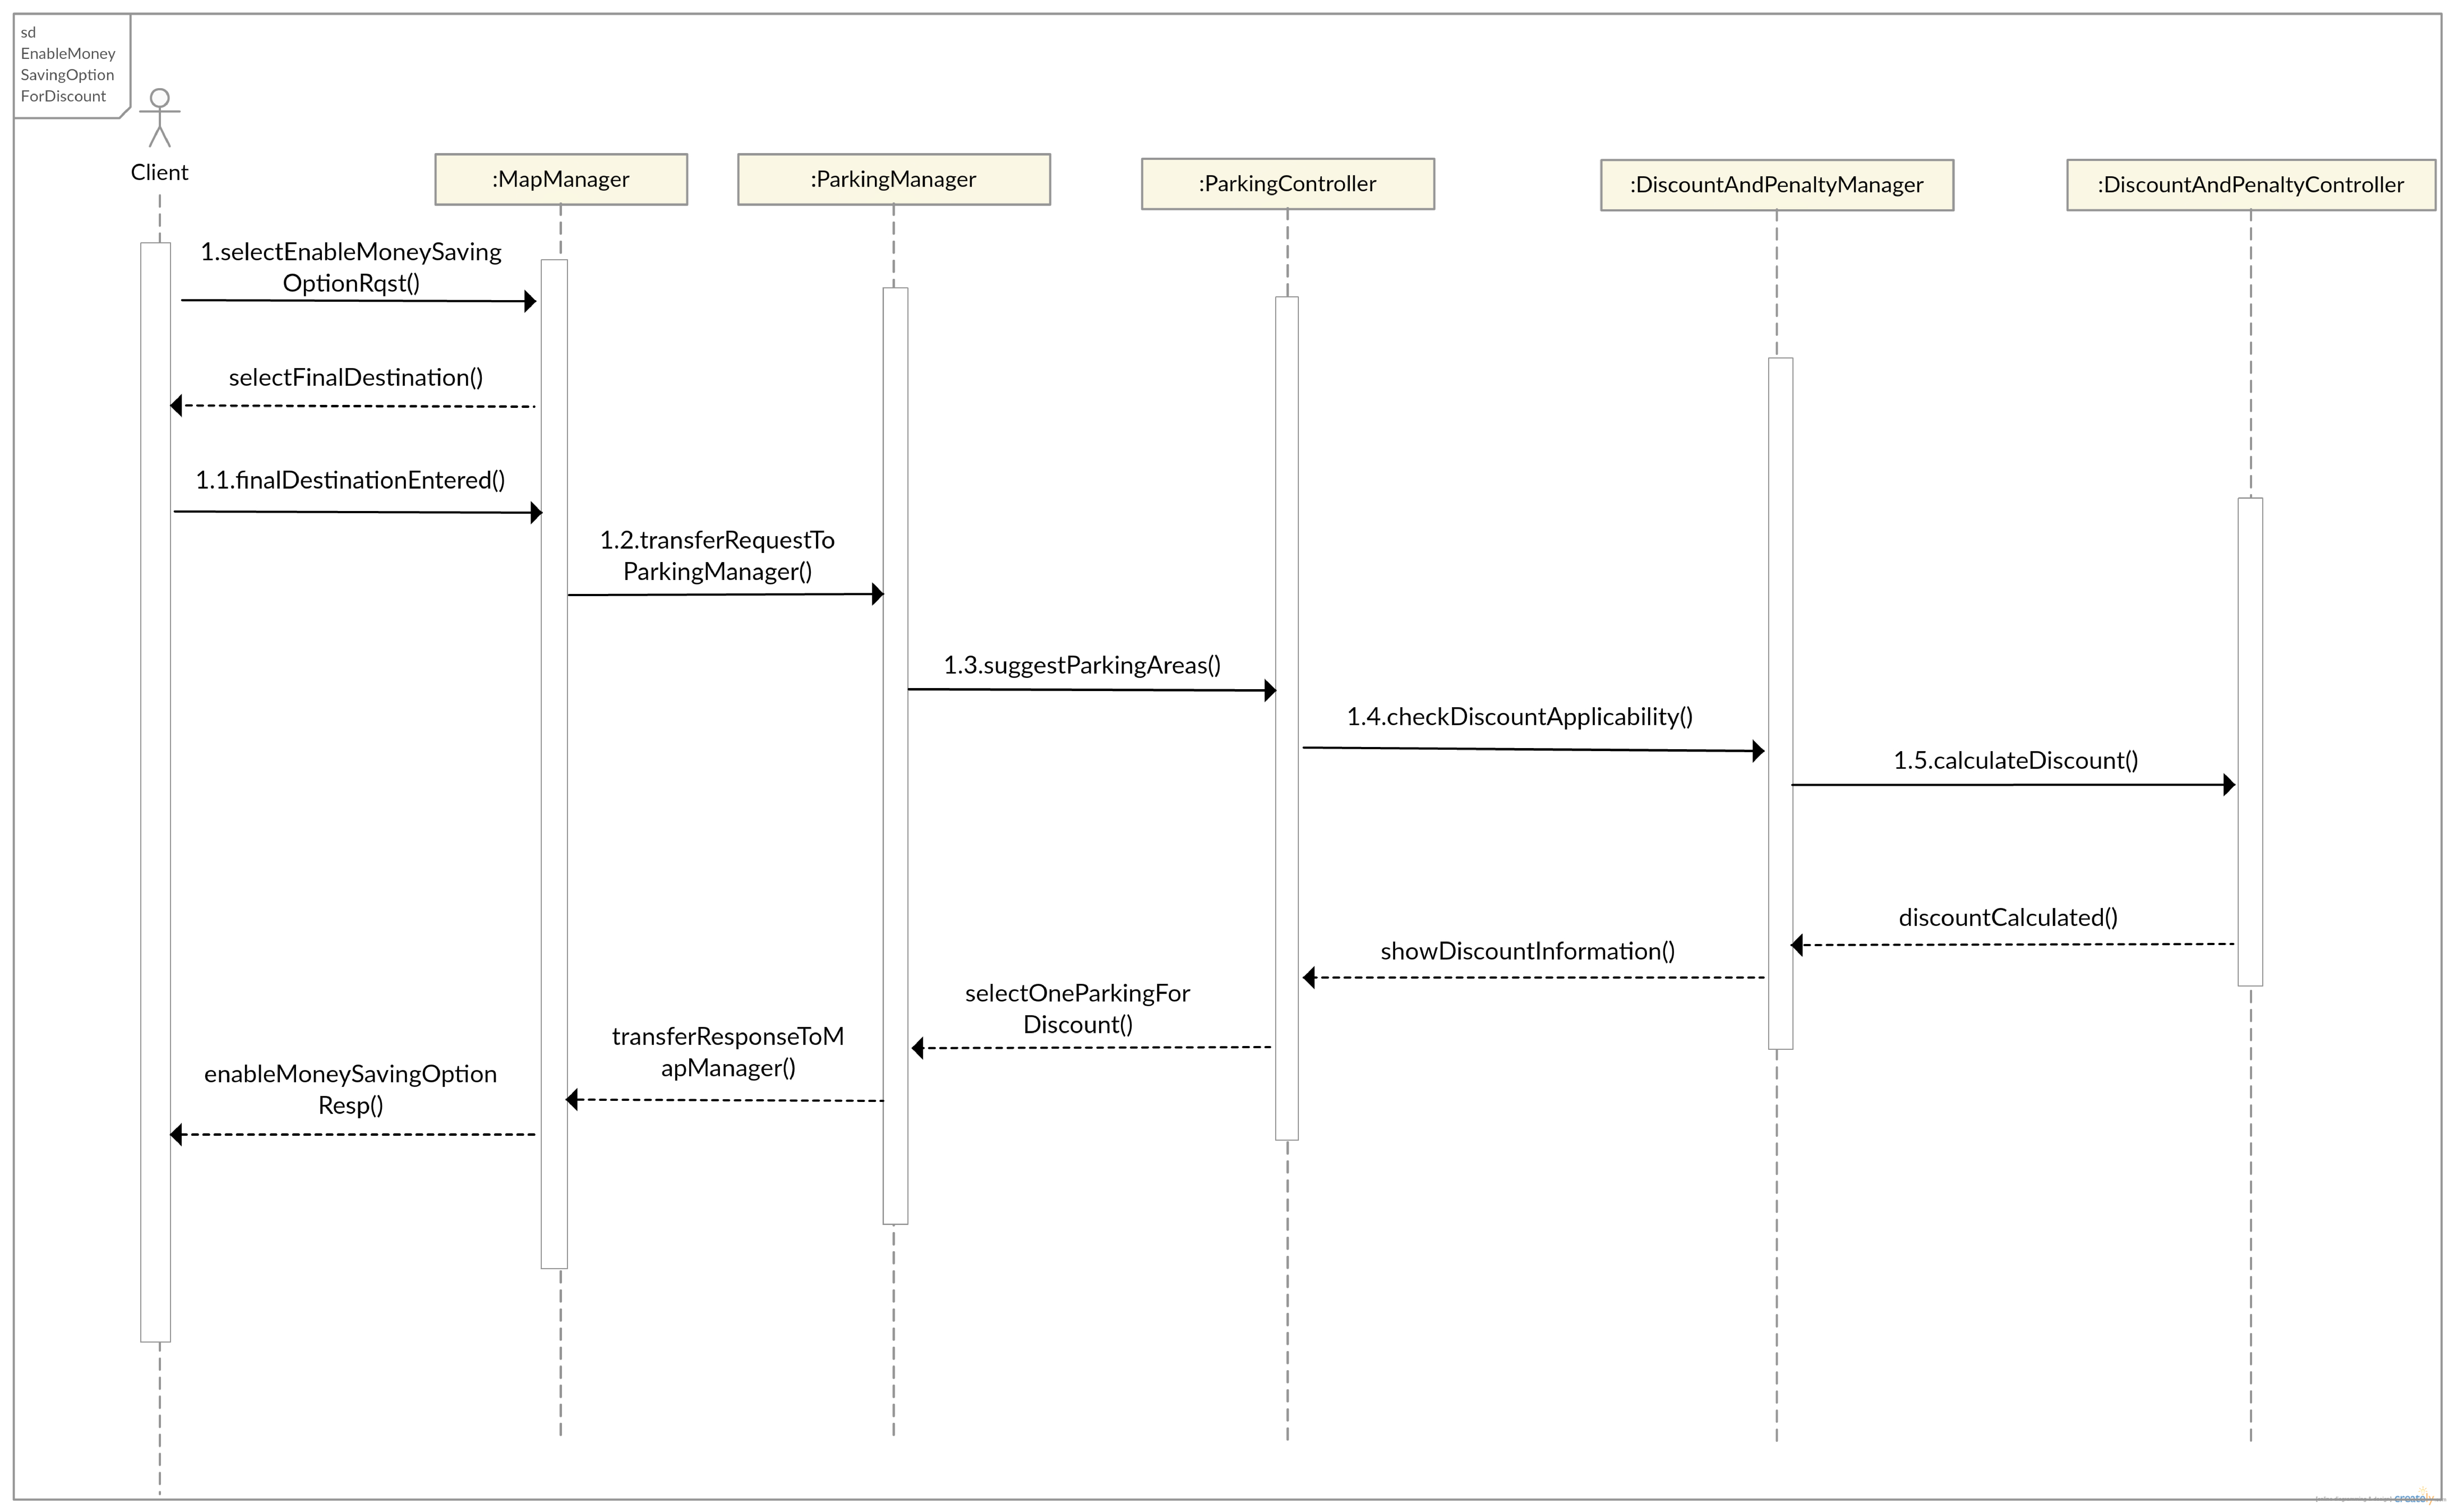
\includegraphics[width=\linewidth,keepaspectratio]{figures/money_saving_option_runtime.eps}
	\caption{Sequence diagram for the activation of the money saving option}
	\label{fig:money_saving_option_runtime}
\end{figure}

The Client/User wants to select/enable money saving option for availing a discount. In order to do that, he/she must select the final destination through the map manager. The map manager asks to select the final destination immediately after selecting the money saving option. After entering the final destination, the request is transferred to the Parking controller through the parking manager to select the parking areas that have a discount.

To check to discount applicability, the parking controller communicates with the discount and penalty manager. The discount controller checks if the parking area is applicable for a discount and calculates the discount. This discount information along with the parking area is sent as a response to the Client/User through the map manager.


\section{Component interfaces}

\section{Selected architectural styles and patterns}

\section{Other design decisions}

\chapter{Algorithm design}
\chapter{User interface design}

\section{Mock-ups}
We have already presented the mock-ups for mobile and desktop versions of the app in section 2.2.1 of the Requirements analysis and specification document.

\section{UX diagrams}
In this section UX diagrams for some of the relevant operations will be showed in order to better describe the user interaction with the system.

\begin{figure}[h]
	\centering
	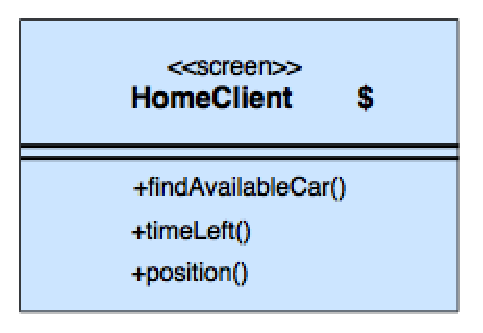
\includegraphics[width=6cm,keepaspectratio]{figures/resv_ux_diagram.eps}
	\caption{UX user with active reservation}
	\label{fig:resv_ux_diagram}
\end{figure}

\begin{figure}[h]
	\centering
	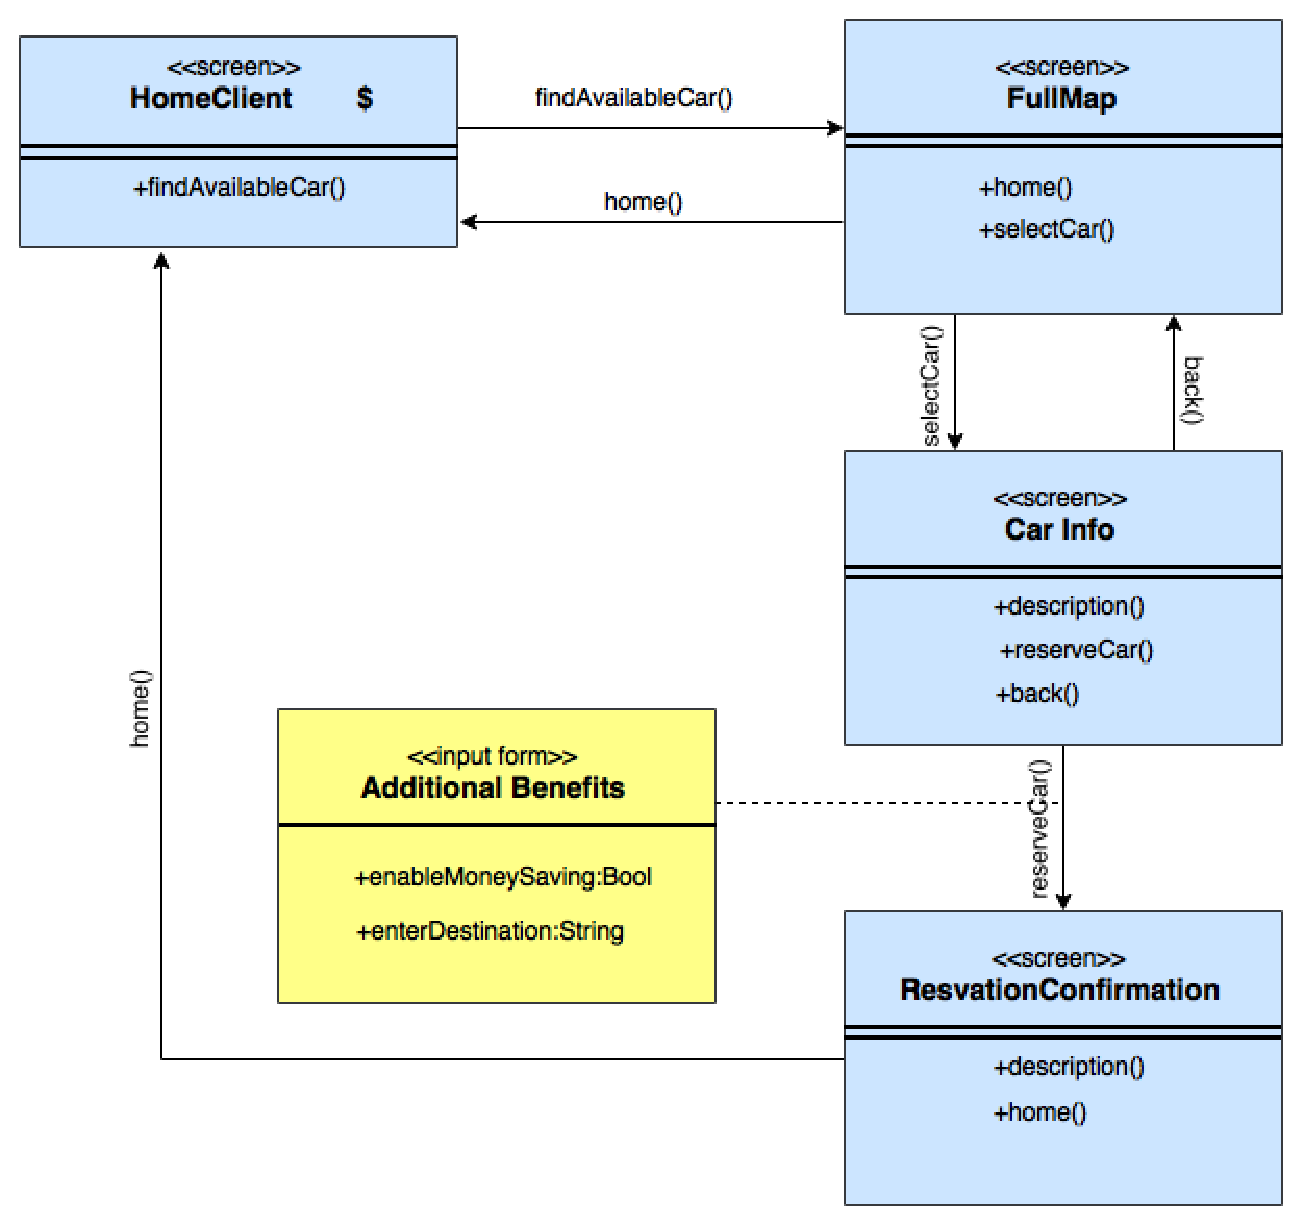
\includegraphics[width=\linewidth,keepaspectratio]{figures/notresv_ux_diagram.eps}
	\caption{UX user with no reservation}
	\label{fig:notresv_ux_diagram}
\end{figure}

\clearpage
\section{BCE diagram}
The figure~\ref{fig:bce_diagram} shows the Business-Controller-Entity diagram for users that access to the homepage not having an active reservation of a car. A BCE diagram is very useful when the MVC pattern is used as arch
\begin{figure}[h]
	\centering
	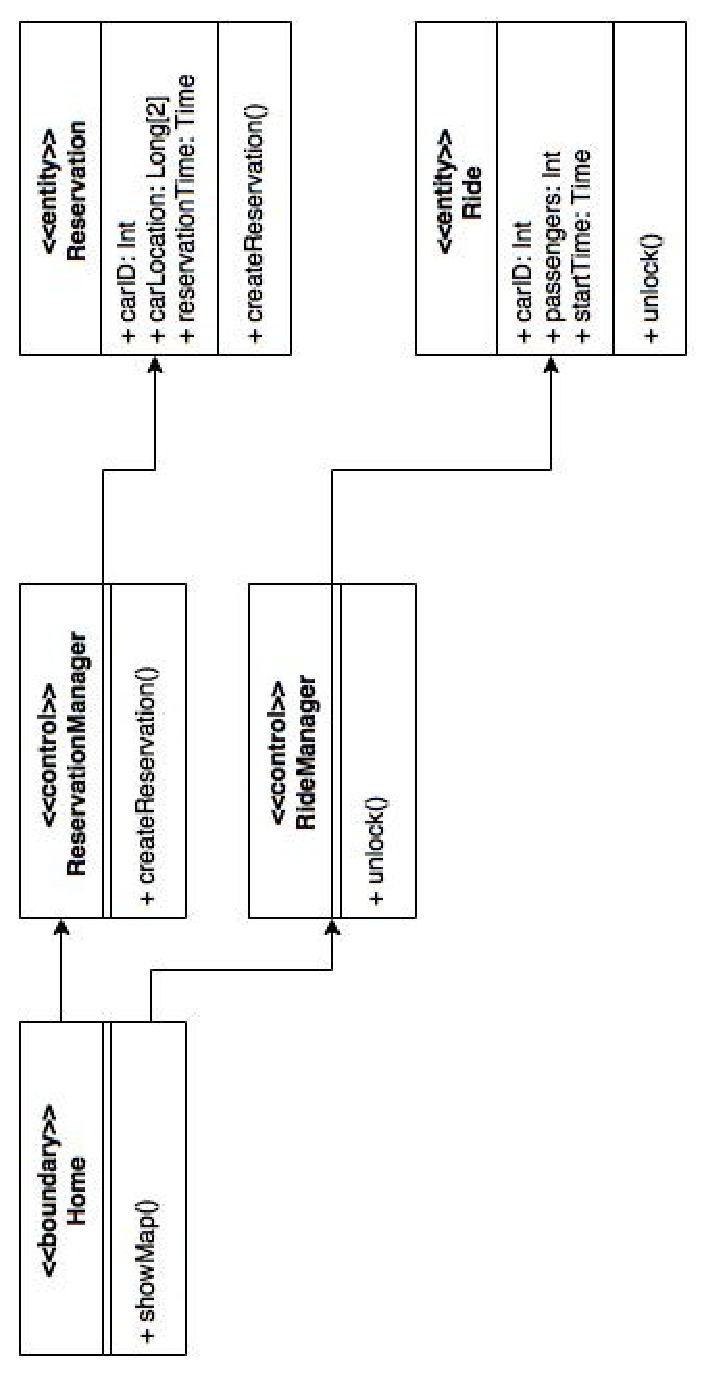
\includegraphics[height=14cm,keepaspectratio]{figures/bce_diagram.eps}
	\caption{BCE user with no reservation}
	\label{fig:bce_diagram}
\end{figure}
\chapter{Requirements traceability}

Each requirement described in the RASD maps to some of the components reported in this document; below the reader will find the list of components involved for every goal of our service.

\begin{itemize}
	\item {[}G1{]} Registration of a user to the system
	\begin{itemize}
		\item Login Manager
	\end{itemize}

	\item {[}G2{]} Finding the locations of the available cars
	\begin{itemize}
		\item Map Manager
		\item Availability Helper
		\item Cars
	\end{itemize}

	\item {[}G3{]} Reservation of a car
	\begin{itemize}
		\item Map Manager
		\item Selection Manager
		\item Reservation Manager
		\item Reservation Controller
		\item Availability Helper
		\item Cars
	\end{itemize}

	\item {[}G4{]} Expiration of reservation and penalization
	\begin{itemize}
		\item Map Manager
		\item Selection Manager
		\item Reservation Manager
		\item Reservation Controller
		\item Availability Helper
		\item Discount and Penalty Manager
		\item Discount and Penalty Controller
	\end{itemize}

	\item {[}G5{]} Entry of registered user into the car
	\begin{itemize}
		\item Map Manager
		\item Ride Manager
		\item Ride Controller
		\item Car
	\end{itemize}

	\item {[}G6{]} Start charging and notifying the registered user
	\begin{itemize}
		\item Map Manager
		\item Ride Manager
		\item Ride Controller
		\item Discount and Penalty Manager
		\item Discount and Penalty Controller
		\item SMS Gateway Interface
		\item SMS Gateway
	\end{itemize}

	\item {[}G7{]} Stop charging the registered user and lock the
	\begin{itemize}
		\item Map Manager
		\item Ride Manager
		\item Ride Controller
		\item Parking Manager
		\item Parking Controller
		\item Discount and Penalty Manager.
		\item Discount and Penalty Controller
	\end{itemize}

	\item {[}G8{]} Safe areas for parking the reserved cars
	\begin{itemize}
		\item Map Manager
		\item Ride Manager
		\item Ride Controller
		\item Parking Manager
		\item Parking Controller
	\end{itemize}

	\item {[}G9{]} Detection of extra passengers and applying discount
	\begin{itemize}
		\item Map Manager
		\item Ride Manager
		\item Ride Controller
		\item Discount and Penalty Manager
		\item Discount and Penalty Controller
	\end{itemize}

	\item {[}G10{]} Detection of the battery status and applying discount
	\begin{itemize}
		\item Map Manager
		\item Ride Manager
		\item Ride Controller
		\item Discount and Penalty Manager
		\item Discount and Penalty Controller
	\end{itemize}

	\item {[}G11{]} Detection of special parking areas and applying discount
	\begin{itemize}
		\item Map Manager
		\item Ride Manager
		\item Ride Controller
		\item Parking Manager
		\item Parking Controller
		\item Discount and Penalty Manager
		\item Discount and Penalty Controller
	\end{itemize}

	\item {[}G12{]} Checking parking and battery constraints and penalization
	\begin{itemize}
		\item Map Manager
		\item Ride Manager
		\item Ride Controller
		\item Parking Manager
		\item Parking Controller
		\item Discount and Penalty Manager
		\item Discount and Penalty Controller
	\end{itemize}
\end{itemize}
\chapter{Effort spent}

\section{Francesco Fabiani}
\begin{itemize}
	\item 21/11/2016: 1h
	\item 23/11/2016: 2h
	\item 26/11/2016: 1h
	\item 28/11/2016: 1h30min
	\item 30/11/2016: 2h30min
	\item 02/12/2016: 2h
	\item 04/12/2016: 1h30min
	\item 05/12/2016: 2h30min
	\item 06/12/2016: 1h
	\item 07/12/2016: 2h
	\item 08/12/2016: 2h30min
	\item 10/12/2016: 2h
	\item 11/12/2016: 1h30min
	\item 12/12/2016: 3h
\end{itemize}

\section{Jagadesh Manivannan}
\begin{itemize}
	\item 20/11/2016: 1h30min
	\item 21/11/2016: 1h
	\item 22/11/2016: 1h30min
	\item 24/11/2016: 1h
	\item 25/11/2016: 2h
	\item 27/11/2016: 2h
	\item 29/11/2016: 1h30min
	\item 01/12/2016: 3h
	\item 03/12/2016: 1h30min
	\item 04/12/2016: 2h
	\item 06/12/2016: 2h
	\item 07/12/2016: 1h30min
	\item 09/12/2016: 2h
	\item 10/12/2016: 3h
	\item 11/12/2016: 2h
\end{itemize}

\section{Niccolò Pozzolini}
\begin{itemize}
	\item 21/11/2016: 1h
	\item 22/11/2016: 1h30min
	\item 24/11/2016: 2h
	\item 26/11/2016: 1h30min
	\item 27/11/2016: 2h
	\item 29/11/2016: 2h
	\item 30/11/2016: 2h30min
	\item 02/12/2016: 1h
	\item 03/12/2016: 1h
	\item 04/12/2016: 2h30min
	\item 06/12/2016: 1h
	\item 08/12/2016: 1h
	\item 09/12/2016: 1h30min
	\item 10/12/2016: 2h
	\item 11/12/2016: 2h
	\item 12/12/2016: 1h30min
\end{itemize}
\chapter{References}

\section{Used tools}
The tools we used to create this DD document are:

\begin{itemize}
	\item \emph{Creately.com}: for design of sequence diagram of Runtime view,Deployment View.
	\item \emph{Draw.io}: version control for the development of this document.
	\item \emph{GitHub}: for design of the UML diagrams-component view, UX diagram.
	\item \emph{TeXstudio}: drafting of this document.
\end{itemize}
\chapter{Changelog}

\section{v1.1}
\begin{itemize}
	\item Updated the component view 
	\item Updated the runtime view of selection of available car
\end{itemize}

\end{document}